\section{Eksperymenty numeryczne}
\label{eksperymenty_numeryczne}

Przeprowadzono szereg eksperymentów numerycznych. W każdym z nich badano jak zależy wyznaczone sterowanie optymalne od warunków początkowych i przyjętych ograniczeń (maksymalne napięcie lub maksymalne wychylenie). Oprócz tego badano również problem sterowania Segwayem dla różnych jego parametrów (np. zmieniając jego moment bezwładności). Dla każdego przeprowadzono eksperymentu zapisywano wygenerowane wykresy, a następnie je ze sobą porównywano.
\paragraph*{}
Pierwszy przeprowadzony eksperyment dotyczył problemu stabilizacji pozycji obiektu. W tym wypadku obiekt początkowo ustawiony był w niestabilnym punkcie równowagi:
\begin{equation}
x_0=\begin{bmatrix}
0\\
0\\
0\\
0\\
0
\end{bmatrix}
\end{equation}
Dla tego eksperymentu przyjęto następujące ograniczenia wychylenia oraz napięcia:
\begin{equation}
\begin{aligned}
\phi_{max}&=\frac{\pi}{18}\\
u_{max}&=8
\end{aligned}
\end{equation}

\begin{figure}[!t]
	\centering
	\subfloat{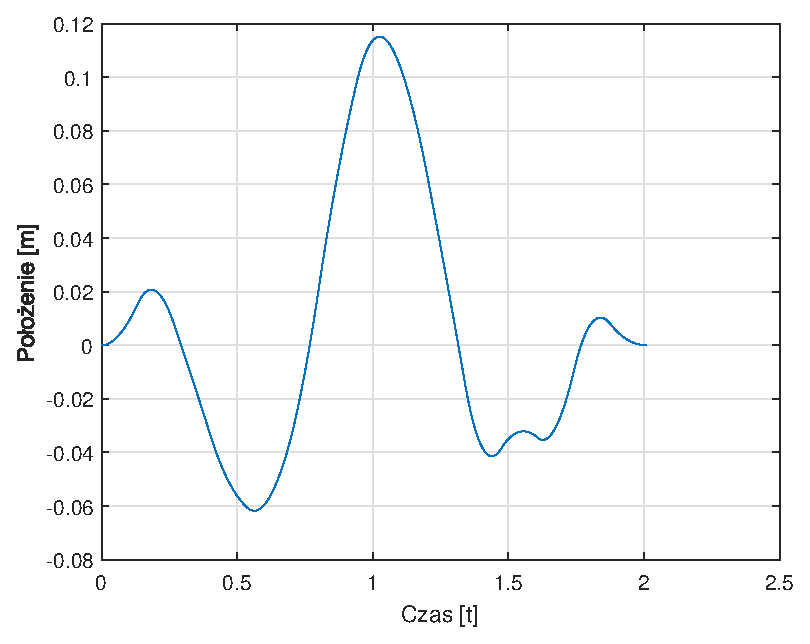
\includegraphics[width=2.8in]{Figures/equ_pos.eps}}
	\subfloat{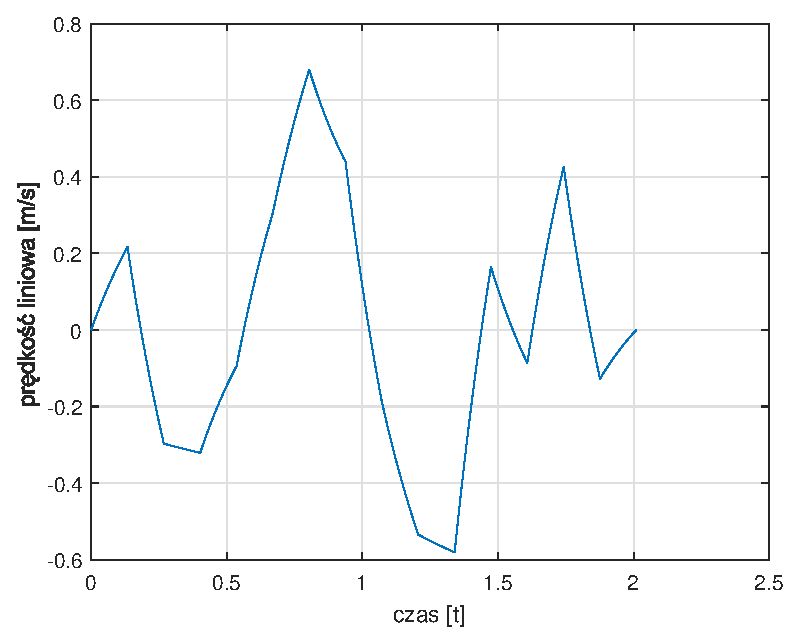
\includegraphics[width=2.8in]{Figures/equ_vel.eps}}
	
	\subfloat{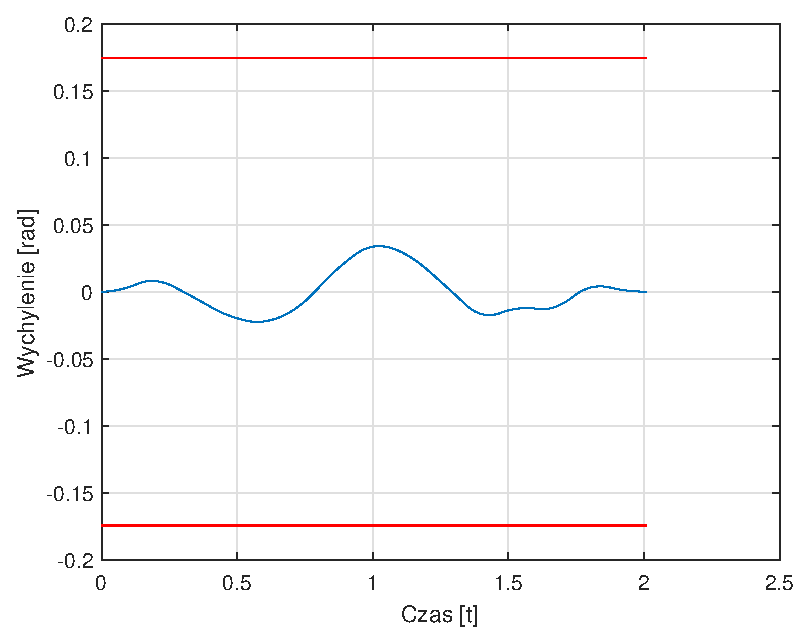
\includegraphics[width=2.8in]{Figures/equ_ang.eps}}
	\subfloat{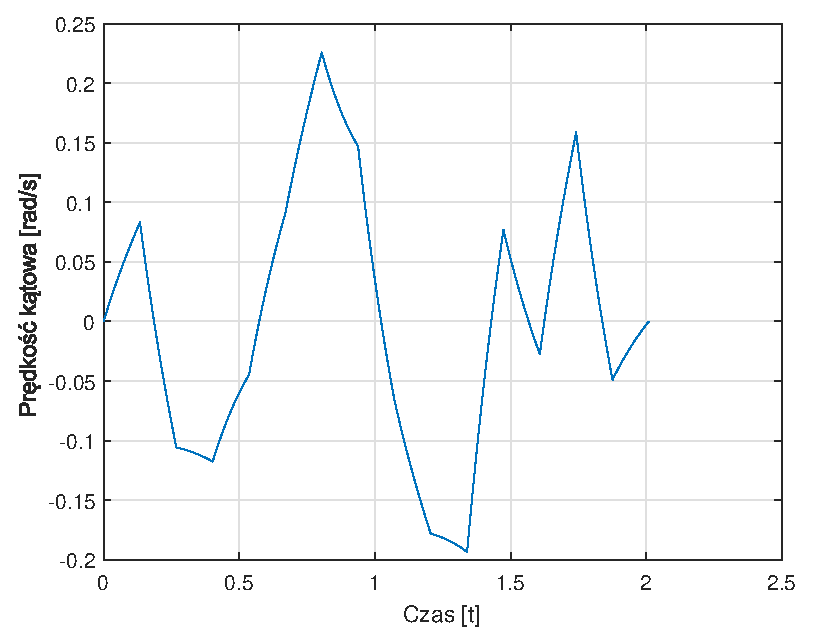
\includegraphics[width=2.8in]{Figures/equ_ang_vel.eps}}
	
	\subfloat{\includegraphics[width=2.8in]{Figures/equ_pen.eps}}
	\subfloat{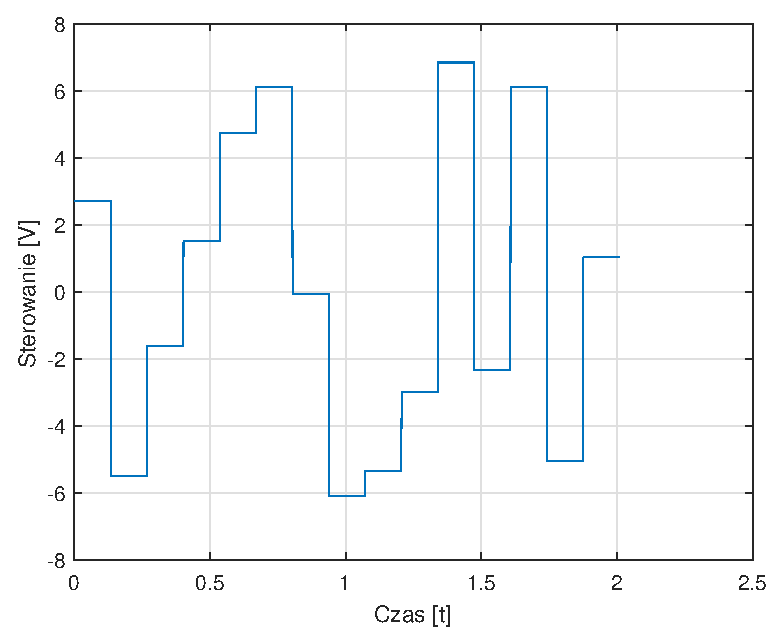
\includegraphics[width=2.8in]{Figures/equ_con.eps}}
	\caption{Zadanie stailizacji obiektu w punkcie równowagi.}
	\label{fig:equ}
\end{figure}